\documentclass[addpoints]{exam}

\usepackage{caption}
\usepackage{graphbox}
\usepackage{hyperref}
\usepackage{multirow}
\usepackage{pythonhighlight}
\usepackage{ragged2e}
\usepackage{subcaption}
\usepackage{tabularx}
\usepackage{titling}
\usepackage{xcolor}

% Header and footer.
\pagestyle{headandfoot}
\runningheadrule
\runningfootrule
\runningheader{CS 201, Spring 2022}{HW 2: Skiplists and Hash Tables}{}
\runningfooter{}{Page \thepage\ of \numpages}{}
\firstpageheader{}{}{}

\qformat{{\large\bf \thequestion. \thequestiontitle}\hfill[\totalpoints\ points]}
% \qformat{{\large\bf \thequestion. \thequestiontitle}\hfill}
\boxedpoints

\printanswers

\graphicspath{{images/}}

\newcommand\colheader[1]{\multicolumn{1}{c}{#1}} % Note: no vertical bars

\title{Homework 2: Skiplists and Hash Tables}
\author{efficient-value}  % <=== Enter your team name.
\date{Habib University\\Spring 2022}

\begin{document}
\maketitle
\part{Analyzing Skiplists and Hash Tables}

The solutions to the problems in this part are to be entered inline below. Remove all the other parts and sections from this document. Enter your team name as the author in the document's title.

\begin{questions}

\titledquestion{A Ranked Set}[10]\footnote{Adapted from Exercise 4.9 in the textbook.}
  Design a version of a skiplist that implements the \texttt{SSet} interface, but also allows fast access to elements by \textit{rank}. That is, it also supports the function \texttt{get(i)}, which returns the element whose rank is \texttt{i} in $O(\log n)$ expected time. (The rank of an element \texttt{x} in an \texttt{SSet} is the number of elements in the \texttt{SSet} that are less than \texttt{x}.)
  Describe how your version differs from a regular skiplist and provide pseudocode of \texttt{find(x)} and \texttt{get(i)} for this version.
  \begin{solution}
  While a regular skiplist would be using index, in this adaptation we would be using rank in place of index.\\
 
      Pseudocode:\\
  \indent \hspace{3em} def get(i): \\ 
  \indent \hspace{3em} n {\#} \textbf{starting node} \\
  \indent \hspace{3em} h {\#} \textbf{height of top list}\\
  \indent \hspace{3em} j = -1 {\#} \textbf{current node position}\\
  \indent \hspace{3em} while height $>=$ 0\\
  \indent \hspace{6em}while i $>$ j + n.length[height]\\
  \indent \hspace{9em}if j + length of rank == i\\
  \indent \hspace{12em}return n.next[height].x {\#} \textbf{returning}\\
  \indent \hspace{9em}else\\
  \indent \hspace{12em}j = j + n.length(height)) {\#} \textbf{current node position}\\
  \indent \hspace{12em}n = n.next[height] {\#} \textbf{access the height of the list}\\
  \indent \hspace{9em}break\\
  \indent \hspace{6em}height = height - 1 {\#} \textbf{going down in list}\\
  \indent \hspace{3em}break\\
  \indent \hspace{3em} return n.next[height].x {\#} \textbf{returning rank}\\
  

  
  refrences: Open Data Structues Pat Morin
  https://opendatastructures.org/ods-python-screen.pdf
    \end{solution}

\titledquestion{Finger Search}[10]\footnote{Adapted from Exercise 4.10 in the textbook.}
  A \textit{finger} in a skiplist is an array that stores the sequence of nodes on a search path at which the search path goes down. (The variable \texttt{stack} in the \texttt{add(x)} code on page 87 is a finger; the shaded nodes in Figure 4.3 show the contents of the finger.) One can think of a finger as pointing out the path to a node in the lowest list, $L_0$.
  
  A \textit{finger search} implements the find(x) operation using a finger, walking up the list using the finger until reaching a node \texttt{u} such that \texttt{u.x < x} and \texttt{u.next = nil} or \texttt{u.next.x > x} and then performing a normal search for \texttt{x} starting from \texttt{u}. It is possible to prove that the expected number of steps required for a finger search is $O(1+\log r)$, where $r$ is the number values in $L_0$ between \texttt{x} and the value pointed to by the finger.

  Design, i.e. provide the necessary pseudo code for, a version of a skiplist that implements \texttt{find(x)} operations using an internal finger. This subclass stores a finger, which is then used so that every \texttt{find(x)} operation is implemented as a finger search. During each \texttt{find(x)} operation the finger is updated so that each \texttt{find(x)} operation uses, as a starting point, a finger that points to the result of the previous \texttt{find(x)} operation.
  \begin{solution}
  Defining a function "find()" with parameters x and u. furthermore we would be required to declare two variables one for keeping an account of upper level  list and index of list of nodes respectively.\\
  

PseudoCode:\\
  \indent \hspace{3em}find(x,u); {\#}\textbf{parameters to find x given a list with node u}\\
  \indent \hspace{3em}index node $=0$ {\#}\textbf{index for node list}\\ 
  \indent \hspace{3em}height $= []$ {\#} \textbf{upper top list}\\
 \indent \hspace{3em} while $x > next[index node].x:${\#} \textbf{if x is greater than the node} \\
   \indent \hspace{6em} while $u.[index node + 1] != Null$ {\#}\textbf{And not equals Null}\\
    \\
    \indent \hspace{9em}index node$ = index node + 1${\#} \textbf{move left}\\
    \indent \hspace{6em}break\\
    \indent \hspace{6em}u = $u.next[index node]$ {\#}\textbf{update u}\\
    \indent \hspace{3em}break\\
    \indent \hspace{3em}while  $height >= 0$ {\#}\textbf{if height is greater than or equals to 0}\\
   \indent \hspace{6em} while $x > u.next[height].x$\\
   \indent \hspace{9em} u$ = u.next[height]$ {\#}\textbf{update u}\\
    \indent \hspace{6em}break\\
    \indent \hspace{6em}height $-= 1$ {\#}\textbf{decreasing height}\\
    \indent \hspace{3em}break\\
    \indent \hspace{3em}return $u.next[height].x$\\
  
  reference: https://www.tutorialspoint.com/finger-searching-in-data-structure\\
  https://opendatastructures.org/ods-python-screen.pdf
  
  \end{solution}

\titledquestion{Cuckoo Hashing}
  \begin{tabularx}{1.0\linewidth}{lX}
  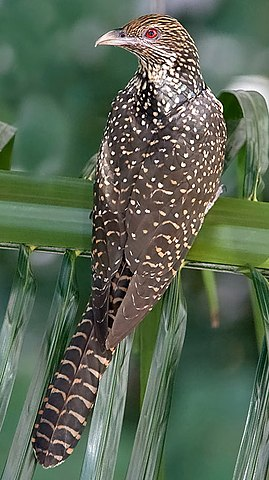
\includegraphics[width=.15\textwidth,align=t]{koel}
    &
      ``Cuckoo hashing is a scheme [...] for resolving hash collisions of values of hash functions in a table, with worst-case constant lookup time. The name derives from the behavior of some species of cuckoo, where the cuckoo chick pushes the other eggs or young out of the nest when it hatches; analogously, inserting a new key into a cuckoo hashing table may push an older key to a different location in the table.'' \cite{wp_cuckoohash} You can read more about cuckoo hashing at \cite{cuckoo_stanford}, \cite{cuckoo_geeks}, and \cite{cuckoo_guide}. Once done, attempt the problems below.
      \vspace{30pt}
      
      Image of Asian Koel, a type of cuckoo, from \cite{wp_koel}.
  \end{tabularx}
  \begin{parts}
  \part[5] Can cuckoo hashing be generalized to use any fixed number of hash tables? What changes do you see in the implementation? Discuss.
  \part[10] Consider a cuckoo hashing scheme using two hash tables of size 10 and using hash functions $h_1$ and $h_2$. Apply this scheme to insert the following sequence of keys to the initially empty tables: $\{29,38,51,41,36,99,123, 9, 4,68,149,59\}$.
    
    The values of $h_1$ and $h_2$ for the keys are given below.
    \begin{center}
      \begin{tabular}{|l||*{12}{c|}}
        \hline
        key, $k$ & 29 & 38 & 51 & 41 & 36 & 99 & 123 &  9 &  4 & 68 & 149 & 59\\\hline\hline
        $h_1(k)$  & 9 & 8 & 1 & 1 & 6 & 9 & 3 &  9 &  4 & 8 & 9 & 9\\\hline
        $h_2(k)$  & 6 & 7 & 2 & 9 & 9 & 0 & 5 &  2 &  1 & 4 & 0 & 2\\\hline
      \end{tabular}
    \end{center}
    
    Indicate the state of the two tables after each insertion.
  \end{parts}
\end{questions}
\begin{solution}
Honestly it wouldn't be wise to make a general cuckoo hashing to work on k number of hash tables. As cuckoo hashing is already 20-30 percent slower than linear probing, as it takes twice the amount of spaces and also causes an increase in the lookup time as it have to go through at least two hash tables atleast.\\
However hash tables could be generalised to use any fixed number of hash tables but for that a great insight is to be required regarding the data that is to be stored. In case of the next part of the same question, an infinite loop is triggered while storing 59, in such cases another hash table might be used so that the loop could break and we wouldn't have to re hash using new hash functions, this process could be iterated if an infinite loop is caused involving the recently added hash table. "A third approach is to slightly modify the cuckoo hash table with a so-called stash, which makes it possible to use nothing more than 2-independent hash functions."\\
reference: https://en.wikipedia.org/wiki/Cuckoo_hashing
\end{solution}
\begin{solution}
According to the rules governing Cuckoo Hashing, we start by placing a key according to their respective key given by h1, in case of collision we push the older value out to the second list according to the key given by h2 while replacing the newer value  first list, in case of a collision again we revert back to the key given by h2. If the collisions still exists (i.e infinite loop) we have to re hash according to a new set of hash functions.\\
Here we are initialising two empty Lists (L1, L2) which are to be populated by given Key (k) according to their respective hash functions h1 and h2.\\
\begin{center}
      \begin{tabular}{|l||*{12}{c|}}
        \hline
        $L1$  &  &  &  &  &  &  &  &   &   &   \\\hline
        $L2$  &  &  &  &  &  &  &  &   &   &   \\\hline
      \end{tabular}
    \end{center}
    Let's start by 29, placing it in it's respective position at h1(20): 9\\
    \begin{center}
      \begin{tabular}{|l||*{12}{c|}}
        \hline
        $L1$  &  &  &  &  &  &  &  &   &   & 29  \\\hline
        $L2$  &  &  &  &  &  &  &  &   &   &   \\\hline
      \end{tabular}
    \end{center}
    Next h1(38): 8\\
    \begin{center}
      \begin{tabular}{|l||*{12}{c|}}
        \hline
        $L1$  &  &  &  &  &  &  &  &   & 38  & 29  \\\hline
        $L2$  &  &  &  &  &  &  &  &   &   &   \\\hline
      \end{tabular}
    \end{center}
    Next h1(51): 1\\
     \begin{center}
      \begin{tabular}{|l||*{12}{c|}}
        \hline
        $L1$  &  & 51 &  &  &  &  &  &   & 38  & 29  \\\hline
        $L2$  &  &  &  &  &  &  &  &   &   &   \\\hline
      \end{tabular}
    \end{center}
    Next h1(41): 1, this results in collsion. So we place h1(41): 1 in L1 and similarly push h2(51): 2 in L2.\\
    \begin{center}
      \begin{tabular}{|l||*{12}{c|}}
        \hline
        $L1$  &  & 41 &  &  &  &  &  &   & 38  & 29  \\\hline
        $L2$  &  &  & 51 &  &  &  &  &   &   &   \\\hline
      \end{tabular}
    \end{center}
    Next h1(36): 6\\
     \begin{center}
      \begin{tabular}{|l||*{12}{c|}}
        \hline
        $L1$  & 41 &  &  &  &  &  & 36 &   & 38  & 29  \\\hline
        $L2$  &  &  & 51 &  &  &  &  &   &   &   \\\hline
      \end{tabular}
    \end{center}
    Next we have collision again so placing h1(99): 9 and pushing h2(29): 6\\
     \begin{center}
      \begin{tabular}{|l||*{12}{c|}}
        \hline
        $L1$  & 41 &  &  &  &  &  & 36 &   & 38  & 99  \\\hline
        $L2$  &  &  & 51 &  &  &  & 29 &   &   &   \\\hline
      \end{tabular}
    \end{center}
    Next h1(123): 3\\
    \begin{center}
      \begin{tabular}{|l||*{12}{c|}}
        \hline
        $L1$  &  & 41 &  & 123 &  &  & 36 &   & 38  & 99  \\\hline
        $L2$  &  &  & 51 &  &  &  & 29 &   &   &   \\\hline
      \end{tabular}
    \end{center}
    Next we have collision again. Placing h1(9): 9 and pushing h2(99): 0\\
    \begin{center}
      \begin{tabular}{|l||*{12}{c|}}
        \hline
        $L1$  &  & 41 &  & 123 &  &  & 36 &   & 38  & 9  \\\hline
        $L2$  & 99 &  & 51 &  &  &  & 29 &   &   &   \\\hline
      \end{tabular}
    \end{center}
    Next h1(4): 4\\
    \begin{center}
      \begin{tabular}{|l||*{12}{c|}}
        \hline
        $L1$  &  & 41 &  & 123 & 4 &  & 36 &   & 38  & 9  \\\hline
        $L2$  & 99 &  & 51 &  &  &  & 29 &   &   &   \\\hline
      \end{tabular}
    \end{center}
    Next we have collison again. Placing h1(68): 8 and pushing h2(38): 7\\
     \begin{center}
      \begin{tabular}{|l||*{12}{c|}}
        \hline
        $L1$  &  & 41 &  & 123 & 4 &  & 36 &   & 68  & 9  \\\hline
        $L2$  & 99 &  & 51 &  &  &  & 29 & 38  &   &   \\\hline
      \end{tabular}
    \end{center}
    Next we have collision again. Placing h1(149): 9 and  pushing h2(9): 2. But we have 51 colliding so we push h1(52): 2\\
    \begin{center}
      \begin{tabular}{|l||*{12}{c|}}
        \hline
        $L1$  &  & 41 & 52 & 123 & 4 &  & 36 &   & 68  & 149  \\\hline
        $L2$  & 99 &  & 9 &  &  &  & 29 & 38  &   &   \\\hline
      \end{tabular}
    \end{center}
    Finally we have 59 causing collision again. Placing h1(59): 9 and pushing h2(149): 0 further pushing h1(99): 9 causing an infinite loop of pushing, it would be resolved if we re-hashed using different hash functions\\
    refrence: https://www.geeksforgeeks.org/cuckoo-hashing/
\end{solution}


\newpage
\part{Implementing a Skiplist}

\begin{figure}[!h]
  \centering
  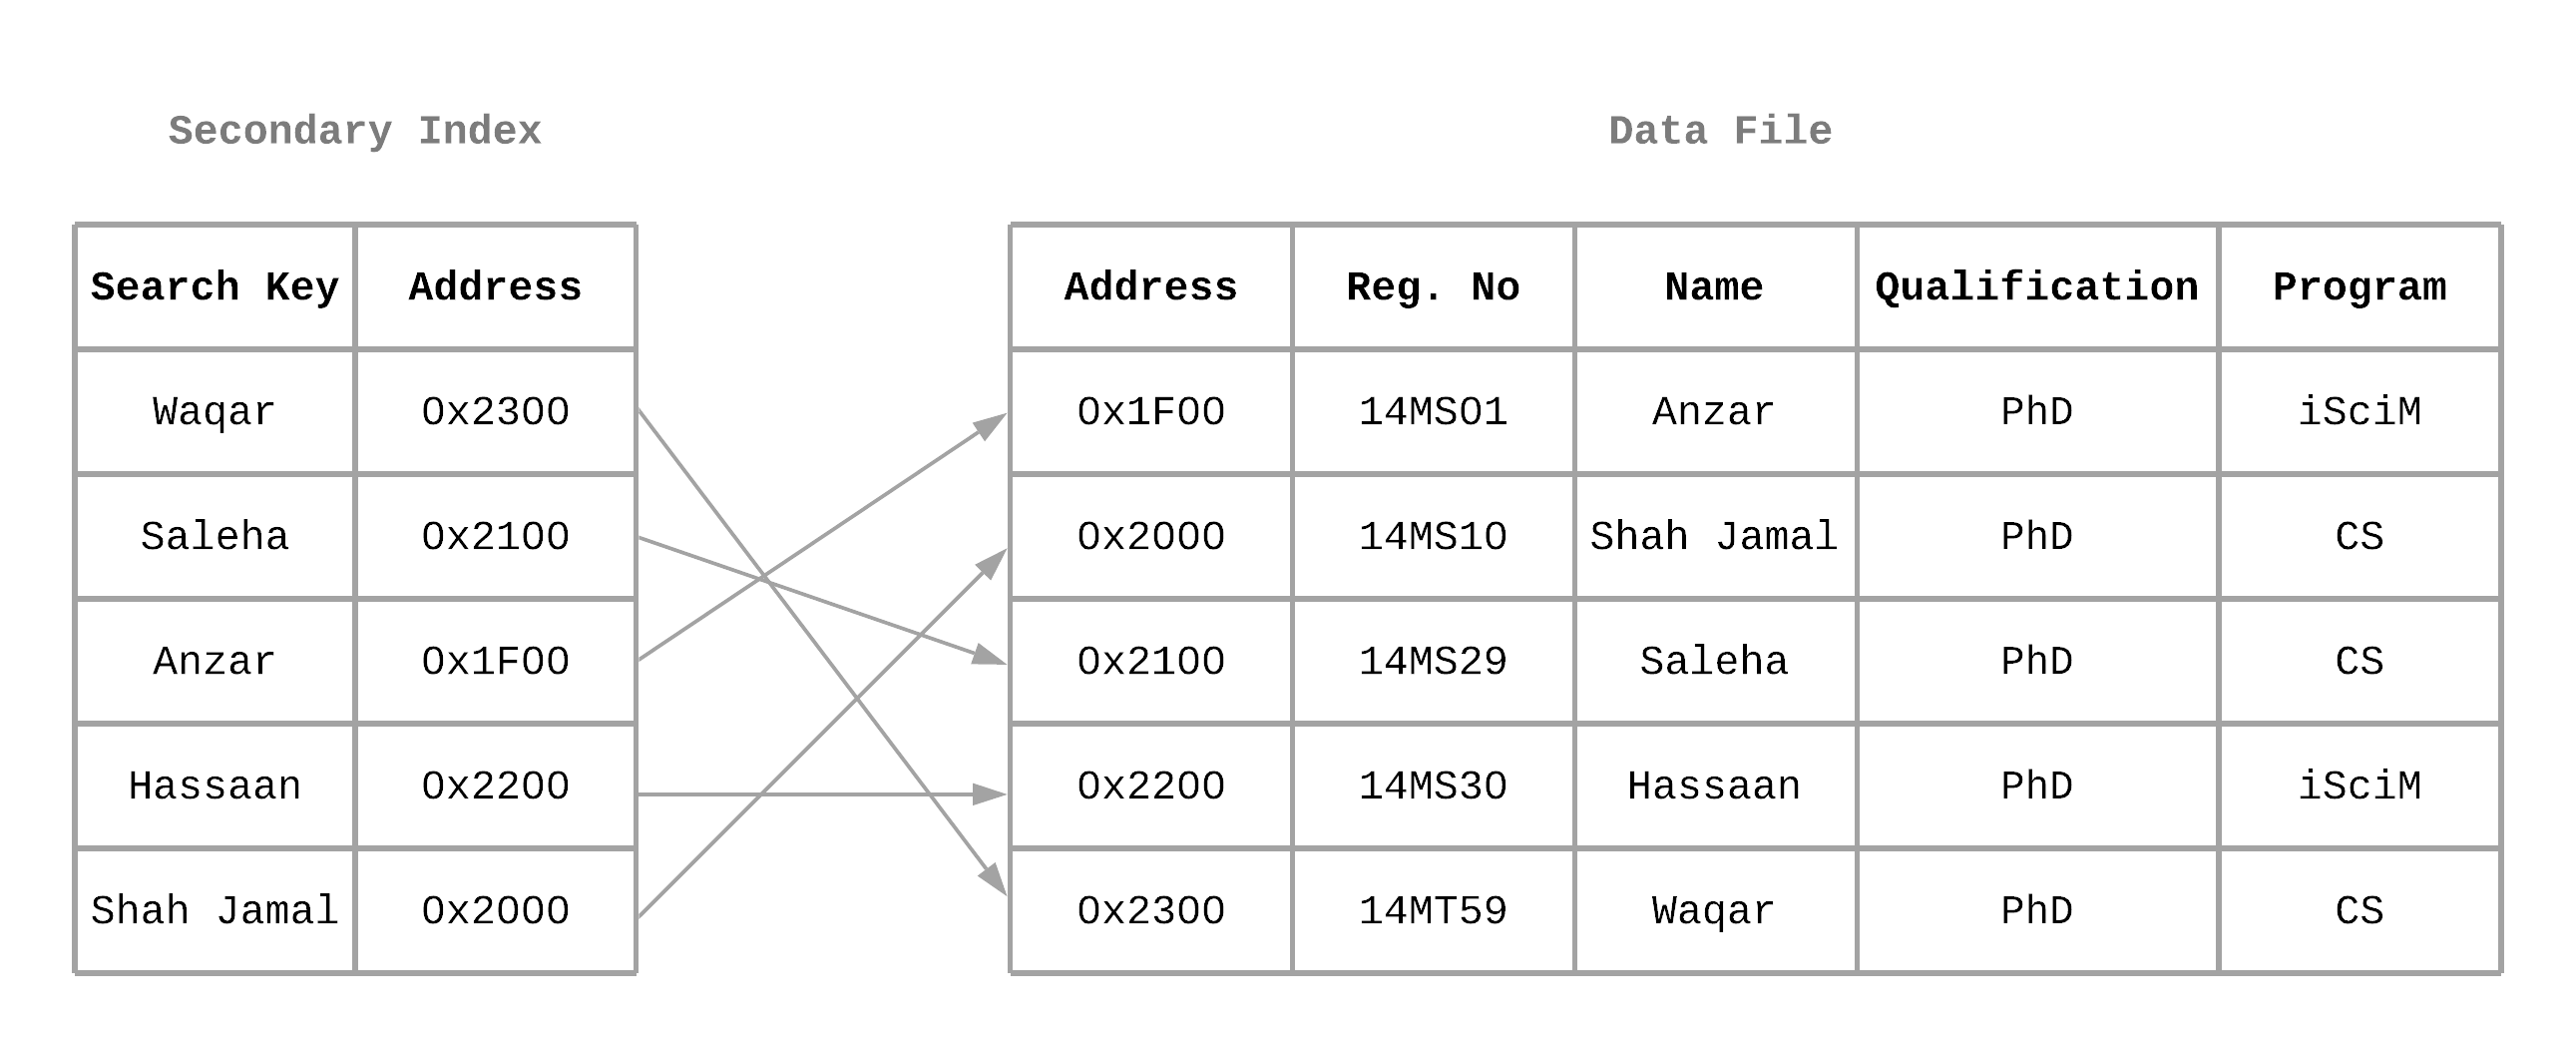
\includegraphics[width=.8\linewidth]{index}
  \caption{An index over the Name attribute of a table. The index stores values of the Name attribute as keys with the associated value being the address of the corresponding record in the table.}
  \label{fig:index}
\end{figure}

You have learned about database indexes in CS 355 Database Systems. Indexes in databases are similar to indexes in books. In a book, an index allows you to find information quickly without reading the entire book. In a database, an index allows the database program to find data in a table without scanning the entire table. An index in a book is a sorted list of words with the page numbers that contain each word. An index in a database is a sorted list of key values with the storage locations of rows in the table that contain the key value. Each key in the index is associated with a particular pointer to a record in the data file. Figure \ref{fig:index} shows an index on the \textit{Name} attribute of an \textit{Instructor} table stored in a data file. Note that key values in the figure are not sorted.
 
The most popular data structure used for indexing in relational databases is Btree (or its variant, such as B+tree). Btrees rose to popularity because they do fewer disk I/O operations to run a lookup compared to other balanced trees. SingleStore is the first commercial relational database in production today to use a skiplist, not a Btree, as its primary index data structure for in-memory data \cite{singlestore}.

You are given a data file, \texttt{data/books.csv}, that contains records of books. Each record contains the following attributes:
\begin{itemize}
\item Book Code
\item Title
\item Category
\item Price
\item Number of Pages
\end{itemize}
For some of the attributes, all the values are unique. Such attributes can be used to index the table. Others have repeating values and are thus unsuitable to be used for indexing.

\section{Implementation Details and Tasks}

You are required to provide the missing implementations for the methods in the files, \texttt{skiplist,py} and \texttt{db.py}, in the accompanying \texttt{src/} sub-folder. \texttt{skiplist,py} contains classes to implement a skiplist. \texttt{db.py} contains a \pyth{Table} class to store records which can be indexed using a skiplist. Every individual field in the \pyth{Table} is stored as strings. Further details are provided in the doc strings in the files. The methods to be implemented are identified with a \pyth{pass} in their body.

  \subsection{Requirement}

  You will need to install the \pyth{typing} module to support certain type hints used in the code.

  \subsection{Tips}

  Below are some tips to avoid the errors that have previously caused tests to fail. Following these may save you many frustrating hours of debugging!
  \begin{itemize}
  \item Store each field that is read from file as a \pyth{str}.
  \item Store a record as a list of field values.
  \item Store a table as a collection of records.
  \item Make sure that the \pyth{Table} can be re-indexed during run-time.
  \item Take care that the keys for the index are the values of the specified attribute. And that the value associated with each key is not the corresponding record, but a means to locate the record in the table.
  \item For the \pyth{select_range} query, think of an approach better than submitting multiple \pyth{select} queries.
  \end{itemize}

  \subsection{Testing}

  Once you have successfully implemented the methods, you can test your code by reading from the accompanying data file, \texttt{data/books.csv}, and performing queries on it. For grading purposes, your submission will be tested automatically by GitHub using the accompnaying \pyth{pytest} file, \texttt{test\_index.py}.

\newpage
\part{Implementing a Hash Table}
  
\begin{figure}[!h]
  \centering
  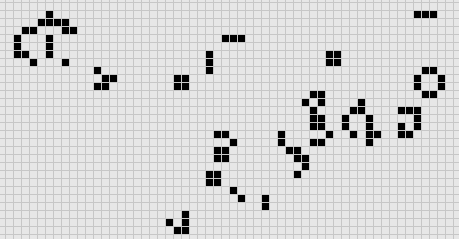
\includegraphics[scale=.8]{banner}
  \caption{A sample game state in Conway's Game of Life, taken from \cite{chaos}.} %
\end{figure}

In this assignment, we will implement 2 different hash tables which differ in their conflict resolution strategy. The hash tables will be further used to implement Conway's Game of Life \cite{wp_gol}.

\section{Game of Life}
\label{sec:imgops}

\begin{quotation}
\href{https://en.wikipedia.org/wiki/Conway's_Game_of_Life}{Conway’s Game of Life} is a simple simulation with surprisingly complex behavior. We start with a simple 2D grid of cells. Each cell can be either alive or dead. The rules are:
\begin{itemize}
\item A live cell stays alive if it has two or three live neighbors.
\item A dead cell becomes alive if it has exactly three live neighbors.
\end{itemize}
We start with a certain set of cell states and then iterate, applying the rules to every cell at each iteration. Despite their simplicity, these rules can produce amazingly complicated behavior.
\end{quotation}
\raggedleft --- A flexible implementation of Conway's Game of Life \cite{gol_impl}
\justify
The rules above are slightly modified from their original formulation so as to be more amenable to our eventual implementation.

\subsection{Initial Configurations}

The game begins with an initial configuration of live cells. This constitutes the starting state of the game. As the rules of the game are deterministic, the starting state completely determines all subsequent states of the game. Some initial configurations result in interesting behavior and have led to the identification of certain classes of patterns.
\begin{description}
\item[Still Life] These patterns are not affected by further iterations of the game and stay unchanged as the game proceeds.
\item[Oscillators] These patterns recur after a fixed number of iterations which are called the \textit{period} of the oscillator.
\item[Spaceships] These are oscillators that change position or \textit{glide} across the grid.
\end{description}

\begin{figure}[!h]
  \centering
  \begin{tabular}{cc}
    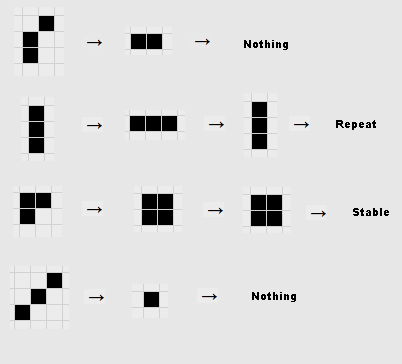
\includegraphics[width=.48\textwidth]{pattern1}
    & 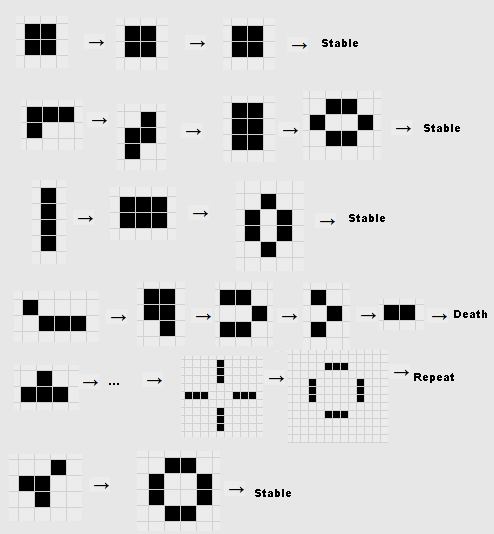
\includegraphics[width=.48\textwidth]{pattern2}
  \end{tabular}
  \caption{Evolution of the game from some initial states, taken from \cite{chaos}.}
\end{figure}


\subsection{Computation}
\begin{quotation}
  It's possible even, to create patterns which emulate logic gates (and, not, or, etc.) and counters. Building up from these, it was proved that the Game of Life is Turing Complete \cite{wp_turing}, which means that with a suitable initial pattern, one can do any computation that can be done on any computer. Later, Paul Rendell actually constructed a simple Turing Machine as a proof of concept, which can be found here \cite{gol_turing}.
\end{quotation}
\raggedleft --- Chaos and Fractals: Conway's Game of Life \cite{chaos}
\justify

\subsection{Visualization}

As the Game of Life is a dynamic system, i.e. its state changes with each iteration, it is best viewed as an animation which this document is unable to present. See Wikipedia \cite{wp_gol} or any of the other pages linked in this document for helpful animations. There are also many inspired and inspiring videos on YouTube including \cite{yt_gol}.

\section{Implementation Details and Tasks}

An implementation of Conway's Game of Life is provided in the accompanying \texttt{src/} folder but is spread over various files containing different classes as follows.
\begin{description}
\item[\texttt{game.py}] provides the \pyth{Game} class and also a \pyth{main()} function to run the game.
\item[\texttt{life.py}] provides the \pyth{Life} and \pyth{Config} classes. \pyth{Life} encodes the state of the game and \pyth{Config} contains various configuration options. Both are used by the \pyth{Game} class.
\item[\texttt{hashtables.py}] provides the abstract classes \pyth{MySet} and \pyth{MyDict} and contains declarations of the classes \pyth{ChainedSet}, \pyth{ChainedDict}, \pyth{LinearSet}, and \pyth{LinearDict} which derive from the abstract classes. You have to implement the derived classes so as to override and implement the interface defined in the abstract classes. These classes are required by the \pyth{Life} class in order to store and update the state of the game.
\end{description}

\subsection{Class details}

\paragraph{\pyth{Life}} Every instance is initialized with a starting configuration which is stored using two different hash tables.
\begin{description}
\item[\texttt{self.\_alive}] stores the two-dimensional $(x,y)$ coordinates of \texttt{live cells}.
\item[\texttt{self.\_nbr\_count}] stores \textit{neighbor information} as key-value pairs where each key is an $(x,y)$ coordinate of a cell with \textit{live neighbors} and its value is the count of its live neighbors.
\end{description}

The hash tables store not only the initial configuration but, once the game starts, they store the state of the game at the end of each iteration. During each iteration, the live cells have to be used to populate neighbor information which in turn must be used to update the live cells for the next iteration. This is already coded in the \texttt{step} method of \texttt{Life}. \textit{Do not modify} the implementation of this class.

\paragraph{\pyth{Game}} It runs a \texttt{Life} instance according to the provided configurations with an option for animation. In the animation system used, the origin, $(0,0)$, is at the top left of the window. This class is provided for your testing. \textit{You may modify} it as per your needs.


All files are fully documented. Please refer to in-file documentation for further details.

\subsection{Task}

Your task is to implement the \pyth{MySet} and \pyth{MyDict} subclass in \texttt{src/hashtables.py} using two different conflict resolution methods. Specifically, you have to implement the following classes which are utilized in the implementation of \texttt{Life}.
\begin{description}
\item[\texttt{ChainedSet}] A hash table that implements the \pyth{MySet} interface using chaining for conflict resolution.
\item[\texttt{ChainedDict}] A hash table that implements the \pyth{MyDict} interface as an associative container and uses chaining for conflict resolution.
\item[\texttt{LinearSet}] A hash table that implements the \pyth{MySet} interface using linear probing for conflict resolution.
\item[\texttt{LinearDict}] A hash table that implements the \pyth{MyDict} interface as an associative container and uses linear probing for conflict resolution.
\end{description}
The conflict resolution strategy to use is indicated through a parameter passed to \pyth{Life} at the time of initialization.

\subsection{Requirements}

You will need to install the following modules.
\begin{description}
\item [\texttt{typing}] to support certain type hints used in the code
\item [\texttt{time}] to support animation of the game
\end{description}

\subsection{Tips}

Below are some tips to gain a better understanding of the homework and facilitate your work for this assignment.
\begin{itemize}
\item Go over the provided implementation in order to understand the role and function of each class and its methods.
\item Run the game using native python types as described below.
\item Run the game using different initial configurations defined in the \pyth{Config} class.
\item Feel free to add other initial configurations defined to the \pyth{Config} class.
\item Feel free to modify the configuration options in \pyth{main()} in order to observe their effect.
\end{itemize}

\subsection{Testing}

You can test the framework by initializing \pyth{self._alive} and \pyth{self._nbr_count} with a native python \pyth{set} and \pyth{dict} instance respectively in \pyth{Life.__init__()}.

Once you have successfully implemented the hashtables, you can test your code by running the provided \texttt{pytest} files. These will also be used by GitHub to auto-grade your submission.
  
\section{Credits}

The Game of Life segment is adapted from \cite{gol_impl}.

\newpage
\begin{thebibliography}{9}

\bibitem{wp_cuckoohash}
Cuckoo hashing, \url{https://en.wikipedia.org/wiki/Cuckoo_hashing}, last accessed on 16 Feb 2022.

\bibitem{cuckoo_stanford}
An Overview of Cuckoo Hashing, Charles Chen, \url{https://cs.stanford.edu/~rishig/courses/ref/l13a.pdf}, last accessed on 16 Feb 2022.

\bibitem{cuckoo_geeks}
Cuckoo Hashing – Worst case O(1) Lookup!, \url{https://www.geeksforgeeks.org/cuckoo-hashing/}, last accessed on 16 Feb 2022.

\bibitem{cuckoo_guide}
Cuckoo Hashing, \url{https://programming.guide/cuckoo-hashing.html}, last accessed on 16 Feb 2022.

\bibitem{wp_koel}
Asian koel, \url{https://en.wikipedia.org/wiki/Asian_koel}, last accessed on 16 Feb 2022.

\bibitem{singlestore}
The Story Behind SingleStore’s Skiplist Indexes, \url{https://www.singlestore.com/blog/what-is-skiplist-why-skiplist-index-for-memsql/}, last accessed on 16 Feb 2022.

\bibitem{wp_gol}
  Conway’s Game of Life, \url{https://en.wikipedia.org/wiki/Conway%27s_Game_of_Life}, last accessed on 16 Feb 2022.

\bibitem{chaos}
  Chaos and Fractals: Conway’s Game of Life, \url{http://pi.math.cornell.edu/~lipa/mec/lesson6.html}, last accessed on 16 Feb 2022.
  
\bibitem{gol_impl}
A flexible implementation of Conway's Game of Life, \url{https://www.refsmmat.com/posts/2016-01-25-conway-game-of-life.html}, last accessed on 16 Feb 2022.

\bibitem{wp_turing}
Turing complete, \url{https://simple.wikipedia.org/wiki/Turing_complete}, last accessed on 16 Feb 2022.

\bibitem{gol_turing}
  This is a Turing Machine implemented in Conway's Game of Life., \url{http://www.rendell-attic.org/gol/tm.htm}, last accessed on 16 Feb 2022.

\bibitem{yt_gol}
epic conway's game of life, \url{https://www.youtube.com/watch?v=C2vgICfQawE}, last accessed on 16 Feb 2022.
\end{thebibliography}

\end{document}
%%% Local Variables:
%%% mode: latex
%%% TeX-master: t
%%% End:

